\documentclass[aspectratio=169]{beamer}
\title{Improvements and current status of the ACTS-based ITk main pass reconstruction}
\author{Andreas Stefl, Noemi Calace, Paul Gessinger-Befurt, Carlo Varni, Pierfrancesco Butti}
\institute{CERN}
\date{2025-08-18}

\setbeamertemplate{navigation symbols}{}

\begin{document}

\frame{\titlepage}

\begin{frame}
\frametitle{Pixel clustering}
\begin{figure}[h]
    \centering
    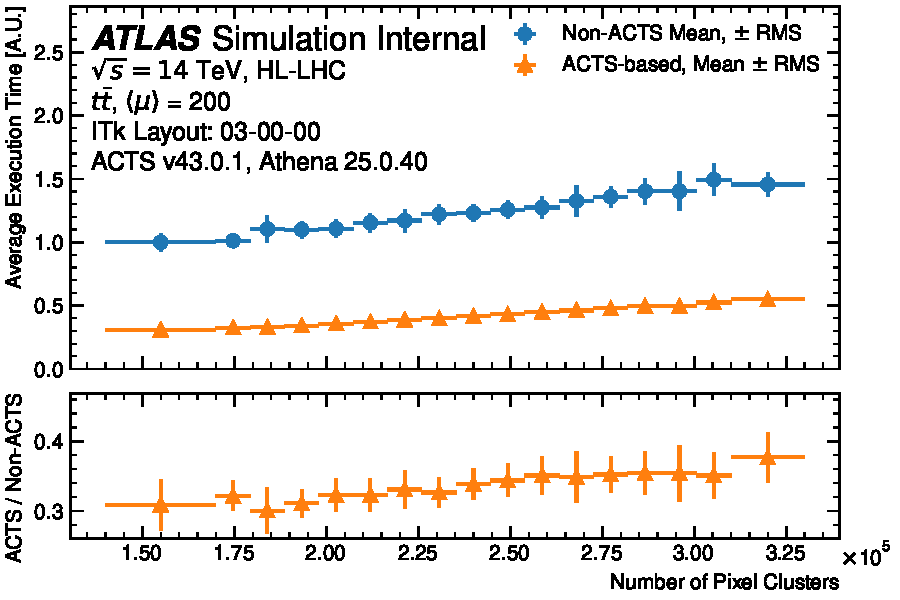
\includegraphics[width=0.8\textwidth]{plots/clustering_pixel.pdf}
\end{figure}
\end{frame}

\begin{frame}
\frametitle{Pixel clustering}
Average execution time (in arbitrary units) of the pixel clustering algorithms as a function of the number of reconstructed pixel clusters, obtained with the current Athena implementation (comparable to the one used for Run 3) and an ACTS-based version. The measurement was taken on the same machine and the same set of $t\bar{t}$ events at $\langle \mu \rangle = 200$ with a center of mass energy of $\sqrt{s}=14$ TeV, using the ITk Layout 03-00-00. An average timing improvement per event of $\sim3\times$ with the ACTS based clustering algorithm is observed while achieving identical physics results.
\end{frame}

\begin{frame}
\frametitle{Strip clustering}
\begin{figure}[h]
    \centering
    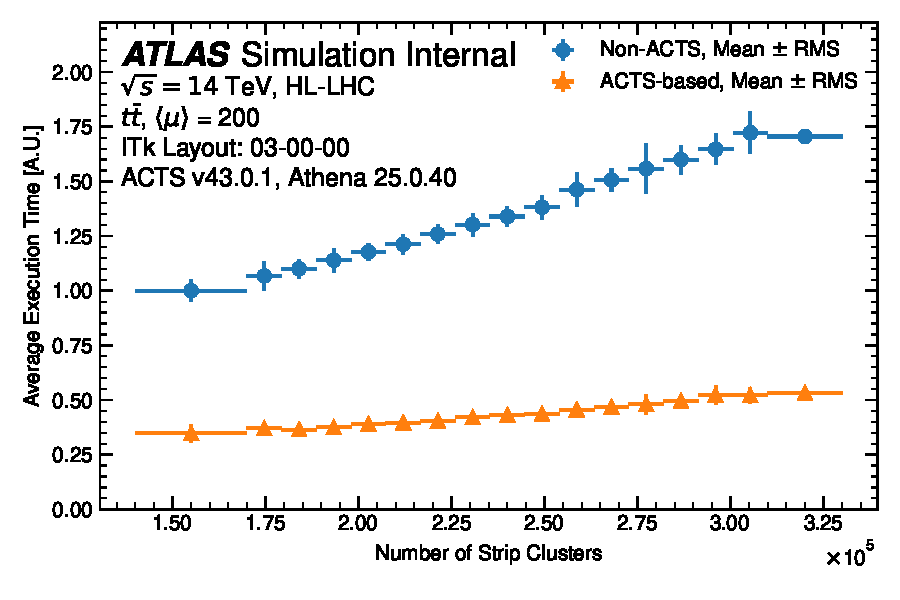
\includegraphics[width=0.8\textwidth]{plots/clustering_strip.pdf}
\end{figure}
\end{frame}

\begin{frame}
\frametitle{Strip clustering}
Average execution time (in arbitrary units) of the strip clustering algorithms as a function of the number of reconstructed strip clusters, obtained with the current Athena implementation (comparable to the one used for Run 3) and an ACTS-based version. The measurement was taken on the same machine and the same set of $t\bar{t}$ events at $\langle \mu \rangle = 200$ with a center of mass energy of $\sqrt{s}=14$ TeV, using the ITk Layout 03-00-00. An average timing improvement per event of $\sim3\times$ with the ACTS based clustering algorithm is observed while achieving identical physics results.
\end{frame}

% \begin{frame}
% \frametitle{Pixel seeding}
% \begin{figure}[h]
%     \centering
%     \includegraphics[width=0.8\textwidth]{plots/seeding_pixel.pdf}
% \end{figure}
% \end{frame}

\begin{frame}
\frametitle{Tracking efficiency}
\begin{figure}[h]
    \centering
    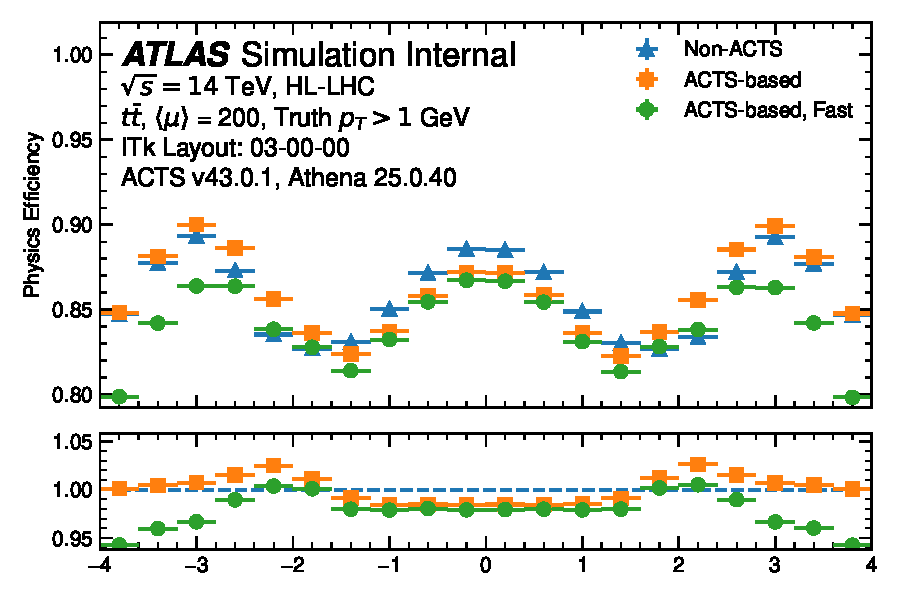
\includegraphics[width=0.8\textwidth]{plots/tracking_efficiency_physics.pdf}
\end{figure}
\end{frame}

\begin{frame}
\frametitle{Tracking efficiency}
Tracking efficiency as a function of the pseudo-rapidity $\eta$ of the associated truth particle using the ITk Layout 03-00-00 for $t\bar{t}$ events at $\langle \mu \rangle = 200$. ACTS-based chains are compared to the current Athena implementation. Lower efficiency is observed in the barrel region $|\eta| < 1.5$. The ACTS-based fast configuration drops further in the endcap region $|\eta| > 2.0$ which is due to CPU optimization trade-offs and under investigation.
\end{frame}

\begin{frame}
\frametitle{Tracking resolution $\sigma(d_0)$}
\begin{figure}[h]
    \centering
    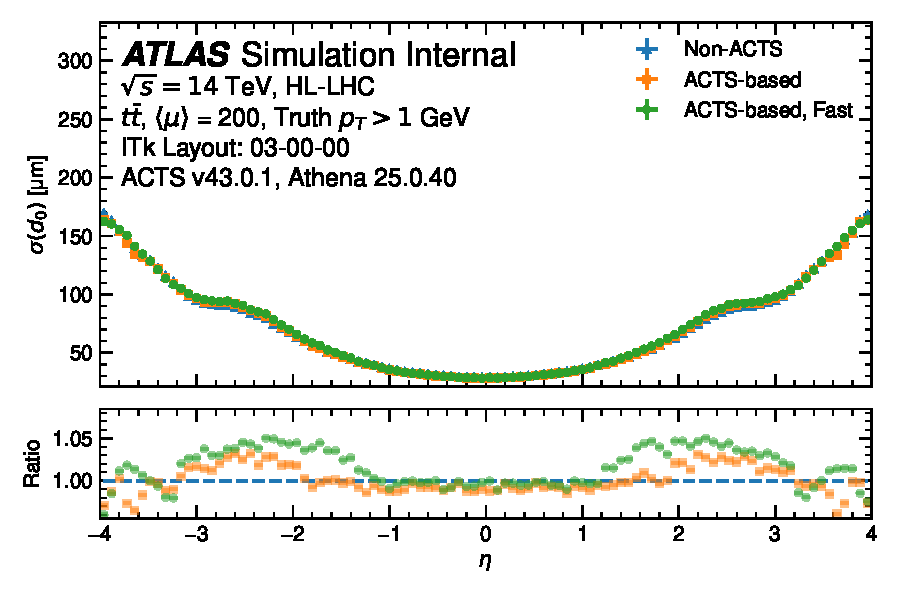
\includegraphics[width=0.8\textwidth]{plots/tracking_resolution_d0.pdf}
\end{figure}
\end{frame}

\begin{frame}
\frametitle{Tracking resolution $\sigma(d_0)$}
Transversal impact parameter $d_0$ resolution as a function of the pseudo-rapidity $\eta$ of the associated truth particle using the ITk Layout 03-00-00 for $t\bar{t}$ events at $\langle \mu \rangle = 200$.
\end{frame}

\begin{frame}
\frametitle{Tracking resolution $\sigma(z_0)$}
\begin{figure}[h]
    \centering
    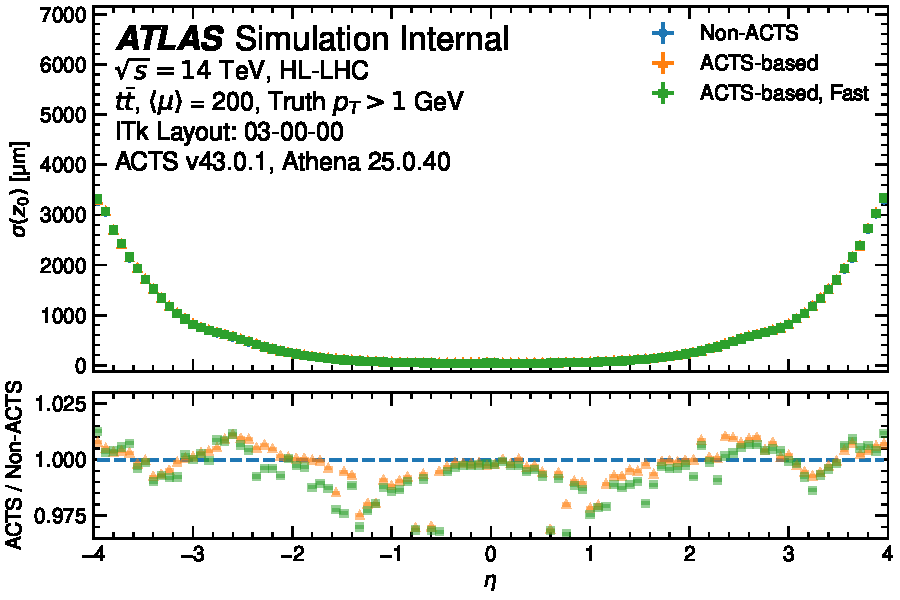
\includegraphics[width=0.8\textwidth]{plots/tracking_resolution_z0.pdf}
\end{figure}
\end{frame}

\begin{frame}
\frametitle{Tracking resolution $\sigma(z_0)$}
Longitudinal impact parameter $z_0$ resolution as a function of the pseudo-rapidity $\eta$ of the associated truth particle using the ITk Layout 03-00-00 for $t\bar{t}$ events at $\langle \mu \rangle = 200$.
\end{frame}

\begin{frame}
\frametitle{Tracking resolution $p_t \ \sigma(q/p_t)$}
\begin{figure}[h]
    \centering
    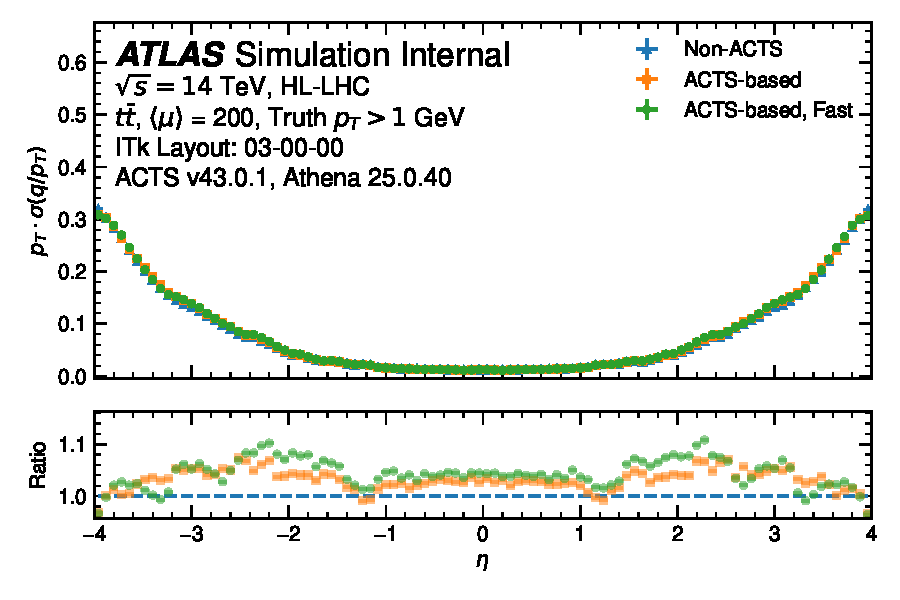
\includegraphics[width=0.8\textwidth]{plots/tracking_resolution_ptqopt.pdf}
\end{figure}
\end{frame}

\begin{frame}
\frametitle{Tracking resolution $p_t \ \sigma(q/p_t)$}
Relative transversal momentum $p_t$ resolution as a function of the pseudo-rapidity $\eta$ of the associated truth particle using the ITk Layout 03-00-00 for $t\bar{t}$ events at $\langle \mu \rangle = 200$.
\end{frame}

\begin{frame}
\frametitle{CPU time evolution}
\begin{figure}[h]
    \centering
    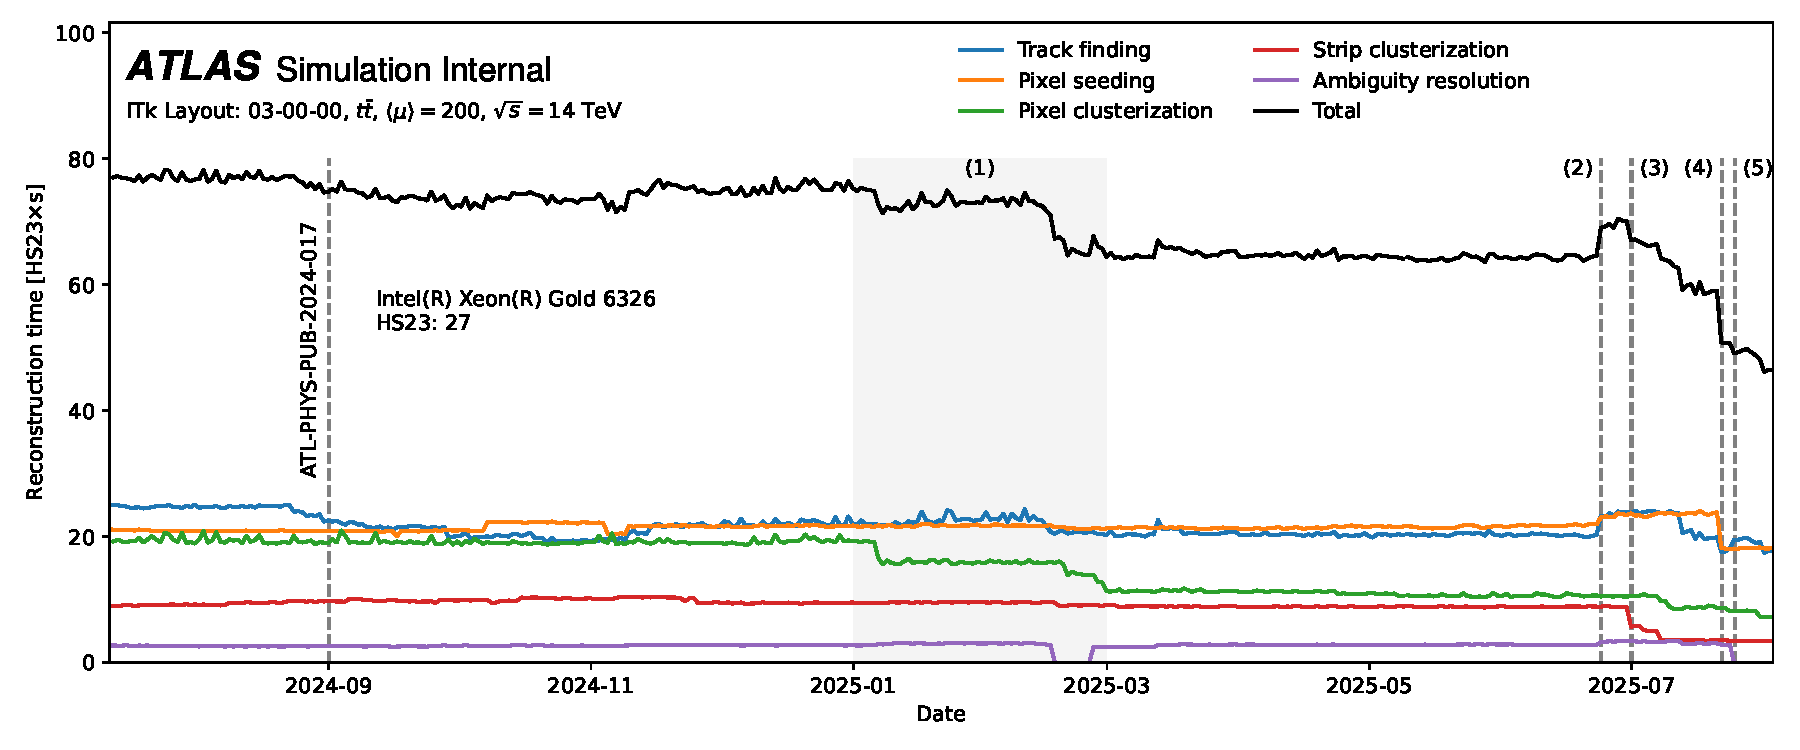
\includegraphics[width=1.0\textwidth]{plots/spot.pdf}
\end{figure}
\end{frame}

\begin{frame}
\frametitle{CPU time evolution}
CPU time evolution of the ACTS-based ITk main pass fast reconstruction, measured on a single core of a Intel Xeon Gold 6148. All measurements were taken on the same machine and the same set of $t\bar{t}$ events at $\langle \mu \rangle = 200$ with a center of mass energy of $\sqrt{s}=14$ TeV, using the ITk Layout 03-00-00. The measured reconstruction time is scaled to HS23$\times$s. On a high level the major changes are: (1) optimizations of the pixel clustering, (2) lowering the $p_T$ reconstruction cut from 1 GeV to 900 MeV, (3) optimizations of the strip clustering, (4) tuning the redundancy of the pixel seeding, (5) merging the ambiguity resolution into the track finding.
\end{frame}

\end{document}
